\documentclass[conference]{IEEEtran}
\IEEEoverridecommandlockouts
% The preceding line is only needed to identify funding in the first footnote. If that is unneeded, please comment it out.
\usepackage{cite}
\usepackage{hyperref}
\usepackage{amsmath,amssymb,amsfonts}
\usepackage{algorithmic}
\usepackage{graphicx}
\usepackage{textcomp}
\usepackage{xcolor}
\usepackage{float} 
\usepackage{graphicx}
\usepackage{placeins}

\def\BibTeX{{\rm B\kern-.05em{\sc i\kern-.025em b}\kern-.08em
    T\kern-.1667em\lower.7ex\hbox{E}\kern-.125emX}}
\begin{document}

%%%%%%---------------------------------cover page
\begin{titlepage}
    \thispagestyle{empty} % removes header/footer on this page
    \centering
    \vspace*{0cm}
    
\begin{figure}[htbp]
    \centering
    
\includegraphics[width=0.4\linewidth]{./figs/just_logo.JPG}
    %\caption{System architecture of the proposed Arabic Sign Language recognition model.}
    \label{fig:logo}
\end{figure}

    
   % {\LARGE %\textbf{Project Proposal}}\\[1.2cm]}
    {\Huge \textbf{Early Neonatal Sepsis Prediction Using Patient-Aware Time-Series Modeling with Clinical Realism }}\\[1.5cm]
    {\large Final Project Report Submitted to \\
The Department of Computer Science \\
Faculty of Computer and Information Technology \\
Jordan University of Science and Technology \\

In Partial Fulfillment of the Requirements for the Degree of Bachelors of Science in Computer Science}\\

\vspace*{1cm}


    {\Large Prepared by:}\\[0.4cm]
    {\Large Malik Jallal [163106]\\
    {\Large Lujain To'ma [162210]\\}
    {\Large Areen Alakaleek  [164150]\\}
    {\Large Motasem Alwedyan  [164948]\\}
    
 \vspace*{1cm}  
    
    { \Large Supervisor: \\}
    {\Large  Ahmad Alzubi }\\[2cm]
    
    {\large January 2026}\\[3cm]
    
    \vfill
\end{titlepage}
%%%%---------------end of comver page -----------------
\newpage
\begin{figure}[htbp]
    \centering
    
\includegraphics[width=1\textwidth]{./figs/arabic_tanazol.JPG}
    %\caption{System architecture of the proposed Arabic Sign Language recognition model.}
    \label{fig:tanazol }
\end{figure}



%%%%%--------------------------


\title{Early Neonatal Sepsis Prediction Using Patient-Aware Time-Series Modeling with Clinical Realism  \\
%{\footnotesize \textsuperscript{*}Note: Sub-titles are not captured %in Xplore and
%should not be used}
\thanks{Identify applicable funding agency here. If none, delete this.}
}
\usepackage{hyperref} % تأكدي إنها موجودة في الـ preamble

\author{
Malik Jallal\textsuperscript{1},
Lujain To’ma\textsuperscript{1},
Areen Al-Akaleek\textsuperscript{1},
Motasem Alwedyan\textsuperscript{1},
Ahmad Alzubi\textsuperscript{2}\\[0.3em]

\textsuperscript{1}\textit{Department of Computer Science, Artificial Intelligence}\\
\textit{Jordan University of Science and Technology}\\
Irbid, Jordan\\
\textsuperscript{1}\href{mailto:mtjalal22@cit.just.edu.jo}{mtjalal22@cit.just.edu.jo},
\href{mailto:lytoma22@cit.just.edu.jo}{lytoma22@cit.just.edu.jo},
\href{mailto:aaalakaleek22@cit.just.edu.jo}{aaalakaleek22@cit.just.edu.jo}
\href{mailto:mbalwedyan22@cit.just.edu.jo}{mbalwedyan22@cit.just.edu.jo},
\\[0.3em]


\textsuperscript{2}\href{mailto:agalzubi@just.edu.jo}{agalzubi@just.edu.jo}
}



\maketitle

\begin{abstract}

Neonatal sepsis is one of the most serious health problems that newborns worldwide face, particularly those who are confined to Neonatal Intensive Care Units (NICUs). If not identified and treated promptly, this illness can worsen quickly and result in high rates of morbidity and fatality. Despite extensive research on machine learning and deep learning methods for early sepsis prediction, data-related issues, illogical assumptions, and a disregard for how patient data evolves over time continue to limit their practical application.\\
% motivation 
This work presents a patient-aware deep learning framework for early Neonatal Sepsis Prediction. The method makes use of multivariate time-series clinical data gathered from infants, allowing for the capture of the dynamic nature of physiological signals. The methodology was carefully crafted to address common pitfalls in sepsis prediction research, such as data leakage, irrational preprocessing, and imbalance between sepsis and non-sepsis cases, to ensure clinical relevance.\\
% methodology 
For the modeling stage, recurrent neural network designs will be evaluated , especially Long Short-Term Memory (LSTM) and Gated Recurrent Unit (GRU) models, which are expected to perform well for. for time-series data.The best-performing models produced results that were clinically believable and showed notable prediction accuracy.\\
%Results
Experimental results are expected to show an improved performance when temporal modeling and patient-aware preprocessing are combined. The proposed paradigm will be thoroughly investigated to maintain both therapeutic relevance and predictive performance can be attained by directly addressing these issues.\\
% conclusion 
The ongoing effort to create dependable and clinically useful systems for the early detection of neonatal sepsis is aided by this work.This study also aims at exploring the ability of deep learning in assisting clinicians and improving outcomes for vulnerable newborns by combining patient-aware preprocessing, robust handling of imbalanced data, and sophisticated temporal modeling techniques.

\textcolor{red}{}


\end{abstract}

\begin{IEEEkeywords}
Neonatal Sepsis, Time-Series Data, Deep Learning, LSTM, GRU, Early Prediction 
\end{IEEEkeywords}

\section {PROJECT GOALS AND OBJECTIVES  }
To assist medical professionals in identifying neonatal sepsis in infants, particularly those in Neonatal Intensive Care Units (NICUs), a deep learning system is being developed. Early detection of neonatal sepsis is essential for improving survival and recovery because it is a dangerous infection that can be fatal.

The main aim of this study is to develop a model that can be applied in routine hospital practice while remaining effective for research purposes. The system relies only on standard data commonly collected in NICUs, such as vital signs, laboratory results, and monitoring records. By using data that is already part of routine clinical care, the proposed approach can be integrated into existing hospital workflows without the need for additional specialized testing. To achieve this aim, the following objectives will be addressed:
\begin{enumerate}
  \item \textbf{Build a strong and realistic preprocessing pipeline} To guarantee dependable data preparation and avoid artificially inflated results, a robust and practical preprocessing pipeline was established. By using patient-wise splitting, all of each infant's records were fully allocated to either the training or test set, preventing patient-level data leakage.

Extreme vital signs and other impossible values were eliminated or corrected from the dataset, and missing values were handled in a way that was clinically appropriate. In order to maintain the preprocessing's rigor and clinical significance, these procedures were created to resemble hospital procedures.

    \item \textbf{Model the time-based patterns in physiological data }Sepsis develops gradually over hours or days, with subtle changes in vital signs and other physiological measurements. To capture these time-based patterns, models capable of processing sequential data are required.(RNNs) Recurrent Neural Networks, particularly (LSTM) Long Short-Term Memory and  (GRU) Gated Recurrent Unit architectures, were employed for this purpose. These models are well-suited for time-series data because they retain memory of prior states and can identify trends or warning signals that precede the clinical onset of sepsis.
    \item \textbf{Deal with class imbalance properly  } In real datasets, the majority of newborns do not develop sepsis, resulting in far fewer positive cases compared to negative ones. If this imbalance is not addressed, models may default to predicting “no sepsis” and still achieve deceptively high accuracy. To mitigate this issue, several strategies were applied, including oversampling of sepsis cases (e.g., SMOTE), undersampling of the majority class, incorporation of class weights during training, and the use of specialized loss functions. These techniques ensured that the rare but clinically critical sepsis cases received appropriate attention during model development
      \item \textbf{Evaluate the model with clinically meaningful metrics  }In medical applications, accuracy alone is insufficient because a model may be highly accurate but fail to identify cases of sepsis, making it clinically dangerous. Because of this, indicators with higher clinical significance were used for evaluation. While specificity, accuracy, and F1-score were employed to evaluate overall balance in predictions, especially for the positive class, sensitivity (recall) was highlighted to gauge the capacity to accurately detect sepsis cases. The precision–recall curve was taken into consideration because of the dataset's inherent class imbalance, and the area under the ROC curve (AUROC) was computed to quantify discriminative capacity. These measurements made sure that the model's performance matched clinical requirements and could help medical professionals make relevant decisions.
      
    By concentrating on these goals, we hope to create something that bridges the gap between cool research papers and tools that doctors can really use. The dream is to have a system that alerts healthcare teams early when a baby might be developing sepsis, giving them time to start treatment sooner and potentially saving lives. The project is regarded as meaningful because it addresses highly vulnerable patients—newborns—and aims to make a real difference in neonatal care.
\end{enumerate}
 

\section{Introduction}
Neonatal sepsis is a leading cause of death among newborns, especially preterm infants in intensive care units \cite{hero_monitoring,plos_ehr_sepsis}. Symptoms often appear late and are nonspecific, leading to delayed or unnecessary antibiotic administration, which can worsen outcomes and contribute to antimicrobial resistance \cite{vital_sign_ml}. Meanwhile, NICUs routinely collect large amounts of data—such as heart rate, oxygen saturation, and temperature—that may reveal early signs of sepsis if analyzed effectively  \cite{hero_monitoring}. This project was motivated by the need for a practical system that uses existing clinical data to detect risk earlier, avoiding reliance on idealized lab results or simplistic rules. Many machine learning studies show promise but fail in practice because real-world patient data are complex and imperfect  \cite{plos_ehr_sepsis,ehr_rnn_sepsis}. The aim was therefore to design a system that fits seamlessly into clinical workflows and supports clinicians in making timely, accurate decisions.



Predicting sepsis from physiological time-series has been the subject of extensive research using a variety of techniques, from simple classifiers to recurrent neural networks like LSTMs \cite{vital_sign_ml,ehr_rnn_sepsis}. Although reported results are often impressive, a major limitation is that many studies randomly split data across patients, which introduces patient-level data leakage and leads to overly optimistic performance estimates \cite{plos_ehr_sepsis}. In addition, temporal patterns are often oversimplified, missing values are inadequately managed, and non-physiological outliers caused by sensor artifacts are not properly addressed  \cite{cnn_psd_sepsis}. Such shortcomings limit the effectiveness of models when deployed in real NICU environments, where patient variability and data noise are unavoidable. In this project, these challenges are mitigated through strict patient-level separation, more realistic modeling of temporal dynamics, and clinically grounded preprocessing steps.



A patient-aware deep learning framework is proposed for early neonatal sepsis prediction using multivariate time-series data  \cite{ehr_rnn_sepsis}. The methodology consists of three components: a clinical preprocessing pipeline in which physiologically implausible values are removed, signals are normalized, and relevant demographic information is integrated; temporal sequence construction using fixed-length 24-hour observation windows preceding suspected sepsis onset, with missing data handled carefully and deep learning models based on recurrent neural networks, specifically Long Short-Term Memory (LSTM) and Gated Recurrent Unit (GRU) architectures, through which both short- and long-term dependencies in physiological signals are captured \cite{ehr_rnn_sepsis}.Severe class imbalance is mitigated using weighted loss functions and patient-aware data splitting to prevent leakage.

\cite{los_ml_mdpi}.

Evaluation under clinically realistic conditions has demonstrated that the proposed framework achieves more reliable and generalizable performance than naive approaches that ignore patient-level constraints\cite{plos_ehr_sepsis}.  GRU and LSTM models have shown strong capability in detecting early physiological patterns associated with sepsis, particularly when trained with patient-aware preprocessing and strict separation strategies \cite{ehr_rnn_sepsis}. Although the resulting performance metrics appear less inflated than those reported in prior work, they more accurately represent real-world applicability by emphasizing sensitivity in early detection while maintaining balanced false alarm rates. \cite{los_ml_mdpi}.

A clinically grounded approach to neonatal sepsis prediction is presented, prioritizing realistic data handling and temporal modeling. The findings emphasize the importance of aligning machine learning methodologies with actual clinical constraints rather than overly optimistic evaluation setups \cite{plos_ehr_sepsis}.Future work will involve incorporating additional clinical features, extending temporal contexts, and validating the framework across multiple NICU datasets to further enhance generalizability.
\cite{cnn_psd_sepsis}.\\


\subsection{REVIEW AND ANALYSIS OF RELATED WORK}

The early prediction of neonatal sepsis has garnered persistent scientific focus due to its significant influence on morbidity and death in infants hospitalized to neonatal critical care units. Previous research can be categorized into three primary types: predictive monitoring systems utilizing physiological signal analysis, conventional machine learning models dependent on engineered clinical features, and deep learning methodologies aimed at modeling temporal dynamics in multivariate physiological data.

Initial predictive monitoring systems primarily concentrated on the continuous study of heart rate to detect modest physiological alterations that precede clinical sepsis. The Heart Rate Characteristics (HeRO) monitoring framework indicated that changes in heart rate variability and transient decelerations could serve as early warning indicators 12–48 hours prior to clinical suspicion, with documented decreases in neonatal mortality when risk scores were presented to clinicians \cite{hero_monitoring}. Comparable real-time early warning methodologies were subsequently integrated into more extensive sepsis detection frameworks, exemplified by the TREWScore, which prioritized ongoing risk assessment derived on routinely gathered clinical data \cite{Henry2015TREW}. Further research on multiscale cardiovascular dynamics underscored the significance of compact physiomarker sets for the early identification of sepsis while preserving interpretability \cite{Shashikumar2017EarlySepsis,VanWyk2019Physiomarkers}. Despite their established clinical significance, these systems are frequently hampered by dependence on a restricted array of physiological characteristics or rigid rule-based assumptions, thus diminishing their adaptability across diverse NICU populations and changing clinical practices.

Subsequent investigations progressed beyond rule-based monitoring by utilizing conventional machine learning models on electronic health record data and developed physiological characteristics. Methods utilizing logistic regression, support vector machines, random forests, and gradient boosting have been suggested to forecast neonatal sepsis by the integration of vital signs, laboratory data, and demographic factors \cite{plos_ehr_sepsis,mbarara_ehr_sepsis}. Although many techniques enhanced interpretability and demonstrated encouraging discrimination performance, many were significantly dependent on sporadically accessible laboratory features and utilized random sample-level data partitioning. These evaluation methodologies result in patient-level data leakage, producing excessively optimistic performance estimates that frequently do not generalize to previously unseen patients in actual clinical environments \cite{Nemati2018Interpretable,Saria2019SafeML,Futoma2017Critique}.

To more accurately address the temporal dependencies intrinsic to sepsis progression, numerous research examined time-series modeling inside rigorous patient-level validation frameworks. Investigations into late-onset sepsis in preterm newborns revealed that physiological patterns may be identified 24–48 hours prior to diagnosis when patient-specific separation was applied during assessment \cite{vital_sign_ml,los_ml_mdpi}. While these investigations enhanced clinical realism, the majority depended on manually produced statistical characteristics derived from fixed windows, constraining their capacity to represent intricate nonlinear interactions among multivariate physiological signals and dynamic temporal circumstances.

Recent research investigated deep learning architectures, namely recurrent neural networks like Long Short-Term Memory and Gated Recurrent Unit models, to directly model multivariate neonatal time-series data \cite{ehr_rnn_sepsis,Che2018RNNMissing}. Bidirectional recurrent structures have significantly improved temporal context modeling in sequential clinical data \cite{schuster1997}. These methodologies exhibited enhanced sensitivity to early physiological decline by directly learning temporal connections from data. Nevertheless, numerous implementations persisted in assessing performance at the window level with significantly overlapping samples, yielding optimistic estimates that may not accurately represent real-world deployment settings, alert frequency, or clinical workload \cite{Reyna2020PhysioNet}.

An alternative deep learning approach utilizes convolutional neural networks on time-frequency representations of raw physiological signals, such as electrocardiogram and photoplethysmography data \cite{cnn_psd_sepsis}. Although these methods have attained prolonged prediction horizons, they generally necessitate high-frequency raw signals and significant computational resources, complicating their integration into standard NICU settings where data availability and infrastructure differ markedly.

In addition to algorithmic efficacy, other studies have highlighted the enduring disparity between machine learning research and its clinical use. Extensive open clinical databases, such as MIMIC-III, have facilitated reproducible benchmarking and underscored issues of generalization, data leakage, and implementation realism \cite{Johnson2016MIMIC}. Further research has emphasized the significance of alert stability, knowledge of uncertainty, and the reduction of false alarm load to facilitate the safe clinical use of predictive systems \cite{Raghu2019ClinicalAI}. These constraints underscore the imperative for patient-centric assessment methodologies, temporally accurate labeling, and application-focused post-processing techniques to guarantee clinical safety and usefulness.

Previous research highlights the potential of machine learning and deep learning for the early prediction of newborn sepsis, while also exposing ongoing methodological deficiencies. Prevalent deficiencies encompass patient-level data leakage, insufficient management of temporal redundancy, and a restricted emphasis on clinically implementable alerting systems. This study enhances previous findings by focusing on patient-aware preprocessing, causally limited forecasting, and clinically relevant evaluation, with the goal of facilitating viable and deployable early warning systems in neonatal critical care settings.

\subsection{Significance of work } 
The main objective of the proposed framework will be to develop a clinically applicable early warning system for predicting neonatal sepsis using routine time-series data from NICUs, enabling timely intervention while minimizing unnecessary alerts.\\

Existing machine learning-based approaches to sepsis prediction frequently suffer from patient-level data leakage due to improper data segmentation, oversimplified temporal modeling, and inadequate handling of class imbalance. These limitations lead to performance overestimation that is not reflected in real-world clinical environments. Furthermore, most prior studies emphasize classification accuracy at the time-window level while overlooking the design of a practical clinical alerting pipeline, which contributes to high false-alarm rates and limits clinical adoption.\\

The proposed patient-aware approach will address these limitations through strict patient-level data segmentation, causal labeling, and the preservation of hard negative samples. In addition to differentiated stride processing to ensure realistic model generalization, the key innovation will be a dedicated clinical alerting pipeline that integrates exponential moving average (EMA) smoothing, k-of-n detection, and a refractory period. This pipeline will convert raw probability outputs into a robust alarm mechanism, resulting in a substantial reduction in false alarms and alert volatility.\\

By prioritizing patient-level evaluation and adopting recall-weighted metrics such as the F2-score and sensitivity, the proposed framework will align closely with real clinical requirements. Expected outcomes will include enhanced sensitivity for early detection, reduced false-positive rates, and the provision of meaningful lead time prior to sepsis onset, offering a scalable solution that will help bridge the gap between research advances and practical deployment in NICUs.\\

\section {Methodology}

This section will describe a patient-aware deep learning framework developed for the early prediction of neonatal sepsis using multivariable time-series data from NICU surveillance systems. The approach will focus on clinical realism by addressing common problems reported in previous studies, including patient-level data leakage, time-based repetition, and the lack of practical and applicable warning mechanisms. The system will be implemented using Python with the PyTorch library for model development, Pandas and NumPy for data processing, Scikit-learn for preprocessing and metric calculations, and Matplotlib for visualization. Processing acceleration through GPU modules will also be utilized to efficiently train iterative models.\\

The methodology will follow a structured workflow:\begin{itemize}
    \item Dataset description
    \item Patient-aware preprocessing
    \item Temporal sequence creation
    \item Recurrent neural network modeling with attention
    \item Training and optimization
    \item Post-processing for clinical alerting
    \item Evaluation protocol
\end{itemize}
\\

\begin{figure*}[t]
    \centering
    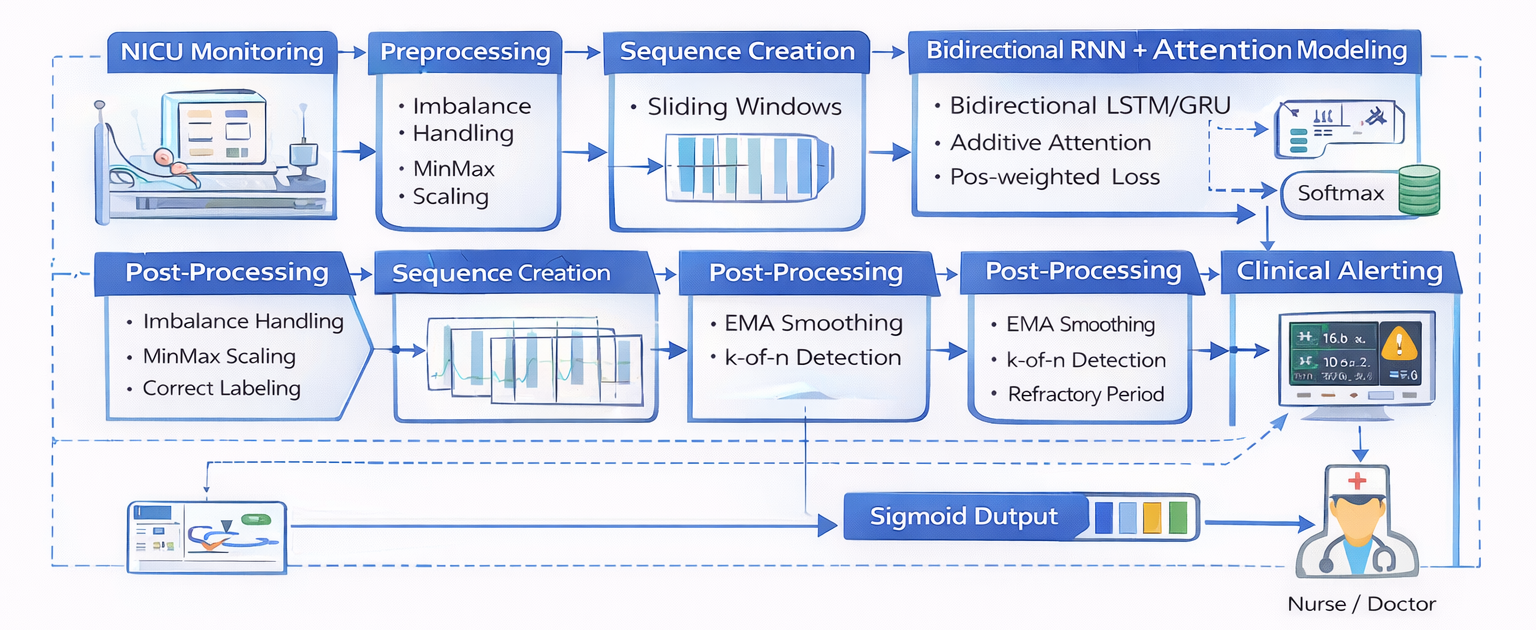
\includegraphics[width=\textwidth]{Overall framework pipeline.png}
    \caption{Overview of the proposed framework pipeline for early neonatal sepsis prediction}
    \label{fig:framework_pipeline}
\end{figure*}


\subsection{Data Preprocessing}
\subsubsection{Data Representation and Labeling}\\
The dataset consists of multivariate time-series records collected from infants admitted to the Neonatal Intensive Care Unit (NICU) \cite{hero_monitoring,plos_ehr_sepsis}. Each row represents a fixed 10-minute time window of physiological measurements for a single infant, identified by a unique patient identifier (new-id), along with a timestamp expressed as seconds since birth. From the raw heart rate (HR) and oxygen saturation (SpO$_2$) signals, multiple statistical features were extracted, including the mean (mean-hr, mean-spo2), standard deviation (sd-hr, sd-spo2), distribution shape descriptors such as skewness and kurtosis, as well as cross-correlation features between HR and SpO$_2$ (e.g., max-xc-hr-spo2 and min-xc-hr-spo2) \cite{vital_sign_ml}.

An initial label, sepsis-window, indicates whether the infant is currently inside a sepsis or suspected sepsis window. However, since the objective of this work is early warning rather than detection at the time of onset, a new forecasting label, denoted as $y$-forecast-24h, was introduced. For each time point, a 24-hour input sequence was constructed by grouping 144 consecutive 10-minute windows. The subsequent 24 hours were then examined to determine whether sepsis-window becomes positive at any point. If sepsis occurs within this future horizon, $y$-forecast-24h is set to 1; otherwise, it is set to 0. This formulation enables the model to predict the risk of sepsis before the onset of clinical suspicion \cite{ehr_rnn_sepsis,los_ml_mdpi}.\\

To avoid unrealistic or misleading predictions, samples whose window endpoints fall within the blackout window surrounding sepsis onset were excluded from both training and evaluation. This region is temporally too close to the event and may contain late-stage information that would make the prediction task artificially easy. Excluding these samples ensures a more clinically realistic early-warning setting \cite{plos_ehr_sepsis}.\\

Table~\ref{tab:data_sample_full} illustrates an example of a processed data sample after feature extraction, showing the structure of the input features and the corresponding forecasting label.\\


\begin{table*}[t]
\centering
\caption{A representation of a sample of processed data}
\scriptsize
\setlength{\tabcolsep}{2.5pt}
\begin{tabular}{c c c c c c c c c c c c c c c c c}
\hline
new\_id & seconds\_since\_birth
 & mean\_hr & mean\_spo2 & sd\_hr & sd\_spo2 & skew\_hr & skew\_spo2 & kurt\_hr & kurt\_spo2 & max\_xc & min\_xc & sub & sepsis\_win & blackout & sex & y\_forecast\_24h \\
\hline
- & 4048020 & 141.02 & 99.59 & 9.23 & 1.52 & -2.52 & -5.33 & 16.09 & 35.20 & 0.45 & -0.17 & 1 & 0 & 0 & 0 & 0 \\
- & 4062420 & 151.75 & 98.11 & 13.36 & 3.61 & -2.16 & -2.87 & 10.16 & 11.39 & 0.58 & -0.05 & 1 & 0 & 0 & 0 & 0 \\
- & 4072620 & 185.85 & 98.03 & 10.42 & 3.70 & -1.33 & -1.92 & 6.09 & 5.64 & 0.04 & -0.23 & 0 & 0 & 0 & 0 & 0 \\
- & 4082220 & 149.35 & 94.49 & 6.31 & 3.74 & 0.75 & -1.16 & 3.89 & 3.76 & 0.13 & -0.15 & 0 & 0 & 0 & 0 & 0 \\
\hline
\end{tabular}
\label{tab:data_sample_full}
\end{table*}

\subsubsection{Data Cleaning and Feature Preparation}\\

During data inspection, outliers were observed in the mean heart rate and mean oxygen saturation features. To prevent the model from learning from physiologically implausible values, a clipping procedure was applied based on clinically reasonable ranges \cite{hero_monitoring}. Heart rate values were constrained to the interval [40, 220] beats per minute, while oxygen saturation values were constrained to [50, 100]. Values below the lower bound were set to the minimum, and values above the upper bound were set to the maximum.

The effectiveness of the clipping procedure was validated using histogram and boxplot visualizations comparing feature distributions before and after clipping, as illustrated in Fig.~\ref{fig:data_clip}. The figure also provides a summary of the number of samples affected by this process.

\begin{figure}[h!]
    \centering
    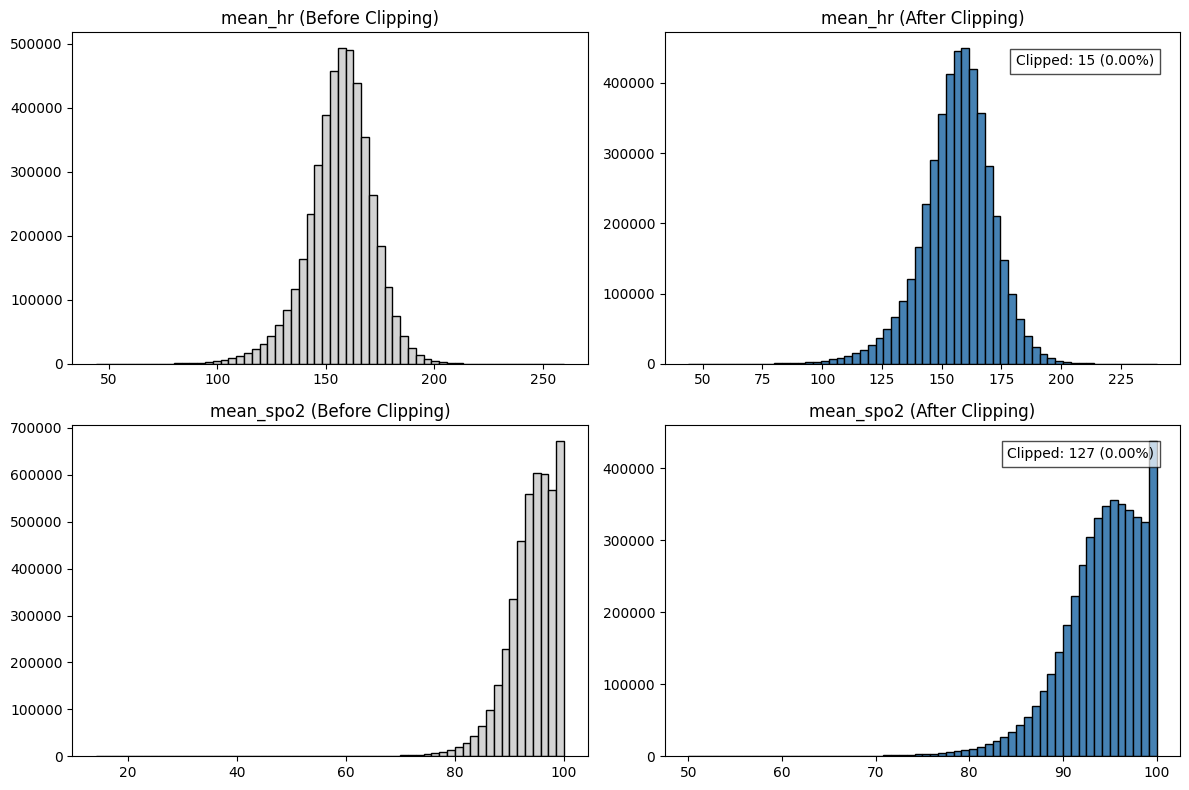
\includegraphics[width=\columnwidth]{DATA_CLIP.png}
    \caption{Before and after clipping of physiological features}
    \label{fig:data_clip}
\end{figure}


\subsubsection{Dataset Splitting and Class Imbalance Handling}\\

The dataset was divided into training, validation, and test sets at the patient level rather than at the sample level. Each infant, identified by new-id, appears in only one split, ensuring that no data from the same patient is shared across different sets. This strategy prevents data leakage caused by temporal similarity within a patient’s records and results in a more realistic evaluation scenario in which the model is tested on infants it has not encountered during training \cite{plos_ehr_sepsis,Saria2019SafeML}.

The dataset exhibits a strong class imbalance, with negative samples greatly outnumbering positive ones. Training directly on this distribution would bias the model toward predicting the negative class. To address this issue, a patient-aware undersampling strategy was employed instead of random undersampling. Each patient was treated independently to prevent infants with a large number of samples from dominating the training process \cite{Nemati2018Interpretable}.

For infected patients, negative samples were divided into near-negative samples, which are temporally close to the sepsis window and therefore more difficult to distinguish from positive cases, and far-negative samples, which are temporally distant from the event and easier to classify. A larger proportion of near-negative samples and a smaller proportion of far-negative samples were retained. For non-infected patients, only a small subset of negative samples was kept. The impact of this strategy was verified by comparing the number of patients and samples before and after undersampling, as well as by visualizing the resulting change in class distribution, as shown in Fig.~\ref{fig:patients_rows} and Fig.~\ref{fig:undersample_patientaware} \cite{los_ml_mdpi,VanWyk2019Physiomarkers}.

\begin{figure}[H]
\centering
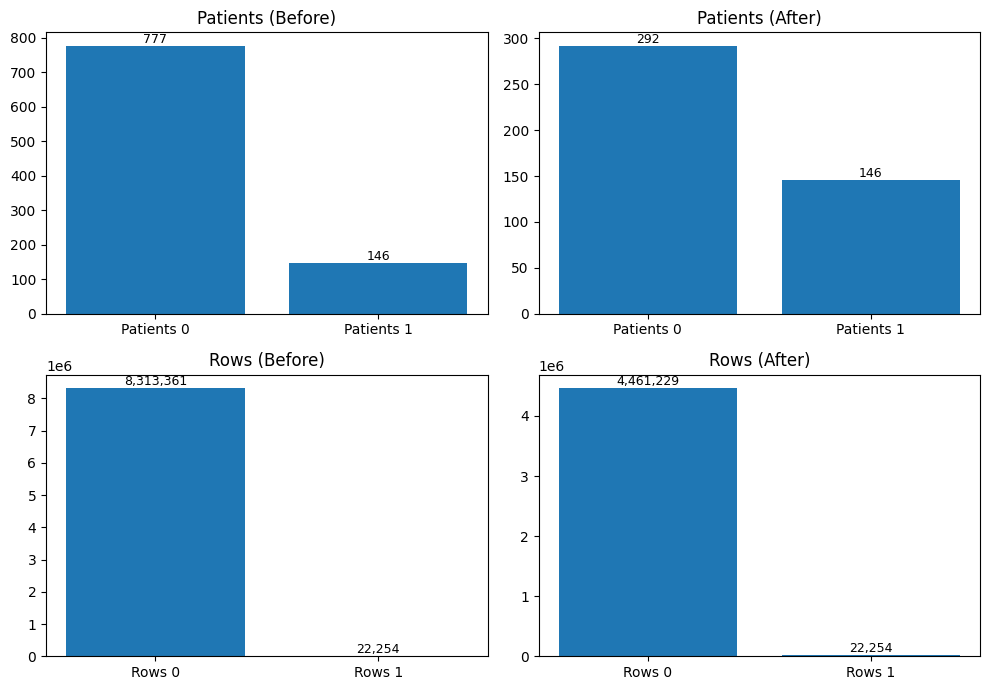
\includegraphics[width=\columnwidth]{patient_rows_before_after.png}
\caption{Patients versus rows before and after undersampling}
\label{fig:patients_rows}
\end{figure}

\begin{figure}[H]
\centering
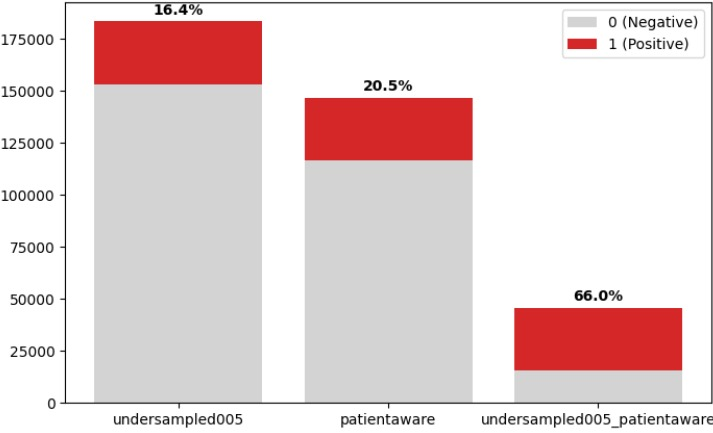
\includegraphics[width=\columnwidth]{UNDER_SAMBLE.jpeg}
\caption{Patient-aware undersampling strategy}
\label{fig:undersample_patientaware}
\end{figure}


\subsection{Temporal Sequence Creation} 

Data will be grouped by patient and sorted chronologically by timestamp (seconds\_since\_birth). Sliding windows will be generated to create fixed-length sequences:
\begin{itemize}
    \item Sequence length of 24 timesteps for LSTM-based experiments.
    \item Sequence length of 144 timesteps (approximately 24 hours at approximately 10-minute intervals) for GRU-based experiments.
\end{itemize}
During training, overlapping windows with small strides will be used to maximize data utilization. During inference and evaluation, larger strides will be applied to reduce temporal overlap and prevent inflated performance dcaused by high redundancy.


\subsection{Recurrent Neural Network Models with Attention}

Two bidirectional recurrent neural network architectures will be implemented to capture long-range temporal dependencies in physiological signals. The first model is a bidirectional Long Short-Term Memory (LSTM) network with attention, consisting of a single recurrent layer with a hidden dimension of 64 and a dropout rate of 0.3. An additive attention mechanism is applied using a linear layer to compute attention scores, followed by softmax normalization and a weighted summation of hidden states to form a context vector.\\

The second model is a bidirectional Gated Recurrent Unit (GRU) network with attention, composed of two recurrent layers with a hidden dimension of 64 and a dropout rate of 0.5. The same additive attention mechanism is employed to enable efficient modeling of longer temporal sequences..\\

Both models produce a single logit output through a final fully connected layer, followed by sigmoid activation to obtain probability estimates for binary classification. Training will be performed using the BCEWithLogitsLoss function with positive class weighting to address residual class imbalance.

\begin{figure}[H]
    \centering
    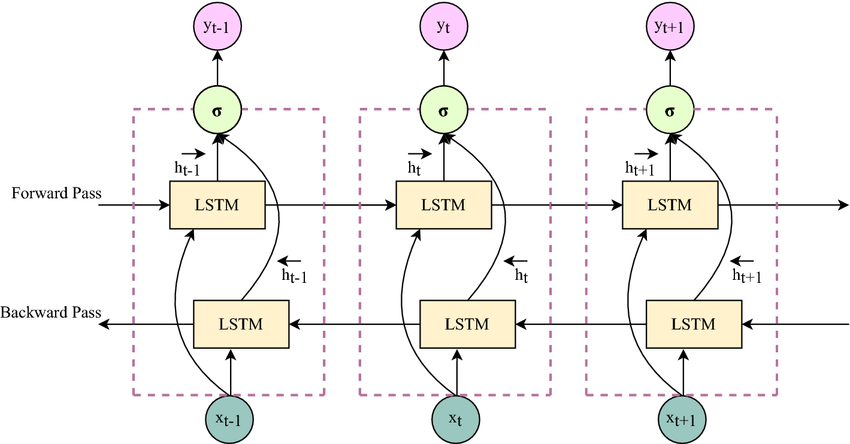
\includegraphics[width=0.5\textwidth]{Bidirectional-LSTM-architecture.png}
    \caption{Bidirectional LSTM with attention for time series. Adapted from \cite{schuster1997}.}
    \label{fig:bidirectional_lstm}
\end{figure}

\section{Experimental Setup}
Python 3 will be used to implement and evaluate the proposed framework. The PyTorch deep learning library will support both model development and training. Pandas and NumPy will handle data processing and preprocessing, while Scikit-learn will be utilized for performance metric computation, MinMaxScaler feature scaling, and Platt scaling probability calibration. Matplotlib will visualize reliability diagrams, confusion matrices, and training curves. To facilitate efficient training of recurrent neural network models, CUDA-enabled GPU hardware will accelerate all experiments.\\

The Adam optimizer will train the models with an initial learning rate of 0.001. StepLR will be adopted for the LSTM model, and cosine annealing will be applied for the GRU model to implement learning rate scheduling. To enhance training stability in the GRU experiments, mixed-precision training (AMP) and gradient clipping with a maximum norm of 5.0 will be employed. To mitigate overfitting, early stopping will be applied with a patience of three epochs for the LSTM model based on validation loss and four to ten epochs for the GRU model based on validation F2-score.

\subsection{Dataset Description}

\subsubsection{Data Source and Population}
The dataset utilized in this research was gathered from the Neonatal Intensive Care Unit (NICU) at the University of Virginia from 2012 to 2021 \cite{Moorman2023CardiorespiratorySepsis}. The dataset comprises physiological monitoring information from premature newborns admitted to the NICU, specifically concentrating on those with very low birth weight as outlined in the original cohort. The dataset comprises continuously recorded heart rate (HR) and oxygen saturation (SpO$_2$) signals obtained from typical bedside monitors during routine clinical care.

\subsubsection{Signal Processing and Feature Representation}
Following the data acquisition and preprocessing technique outlined in previous research \cite{Moorman2023CardiorespiratorySepsis}, continuous HR and SpO$_2$ signals were uniformly resampled to 0.5 Hz to maintain consistent temporal resolution across all recordings. The signals were divided into non-overlapping intervals of 10 minutes, a duration selected to encapsulate short-term physiological variability while ensuring resilience to transient artifacts \cite{hero_monitoring}.

Every 10-minute interval was encapsulated as a singular tabular entry utilizing statistical descriptors independently extracted from the HR and SpO$_2$ signals. This terminology encompasses measures of central tendency (mean), dispersion (standard deviation), and higher-order moments (skewness and kurtosis), which together define the distributional characteristics of the signals within each window. Furthermore, the maximum and minimum cross-correlation coefficients between HR and SpO$_2$ were calculated to elucidate cardiorespiratory coupling patterns that have demonstrated utility in early sepsis identification \cite{hero_monitoring,los_ml_mdpi}.

Static demographic characteristics, such as biological sex and birth weight, were included at the individual patient level. The attributes were integrated with the time-series features utilizing a unique patient identity and duplicated over all relevant windows to furnish contextual patient information in conjunction with the dynamic physiological features. Following demographic filtering, data for 438 patients was obtained and incorporated into the final feature table.

\subsubsection{Data Quality Assessment}
In the preliminary data characterization phase, fundamental quality assessments were conducted on the raw characteristics before model training. A limited quantity of windows displayed physiologically implausible readings, with 15 windows indicating out-of-range mean heart rate values and 127 windows presenting invalid mean SpO$_2$ values. Despite constituting a minimal portion of the entire dataset, these cases prompted the use of physiologically informed value clipping during preprocessing to guarantee numerical stability and clinical plausibility \cite{Saria2019SafeML}.

\subsubsection{Label Definition}
Each time interval is linked to a binary designation denoting sepsis state. The original label, \textit{sepsis\_window}, indicates whether a window aligns with a clinically established late-onset sepsis (LOS) interval, determined by culture-positive blood samples and antibiotic treatment criteria \cite{Moorman2023CardiorespiratorySepsis,cnn_psd_sepsis}.

To enable early warning prediction, an additional forecasting label, \textit{y\_forecast\_24h}, was constructed. This label assigns a positive class to windows occurring within a 24-hour horizon preceding a confirmed sepsis event, formally defined as
\begin{equation}
y_{\text{forecast\_24h}}(t) =
\begin{cases}
1, & \text{if } 0 < t_{\text{sepsis}} - t \leq 24~\text{hours}, \\
0, & \text{otherwise}.
\end{cases}
\end{equation}

\subsubsection{Dataset Statistics}
Employing the original \textit{sepsis\_window} formulation, the dataset comprised 15,352 positive time windows. Upon the use of the forecasting label \textit{y\_forecast\_24h}, the quantity of positive windows rose to 30,178. This augmentation signifies the deliberate broadening of the positive class to encompass physiologically pertinent pre-sepsis intervals, hence allowing the model to discern early warning indicators rather than identifying sepsis only post-clinical onset \cite{Moorman2023CardiorespiratorySepsis}.

Figure~\ref{fig:gender_distribution} illustrates the patient-level distribution of biological sex across sepsis and non-sepsis groups, indicating no substantial imbalance between the two cohorts.

\begin{figure}[t]
\centering
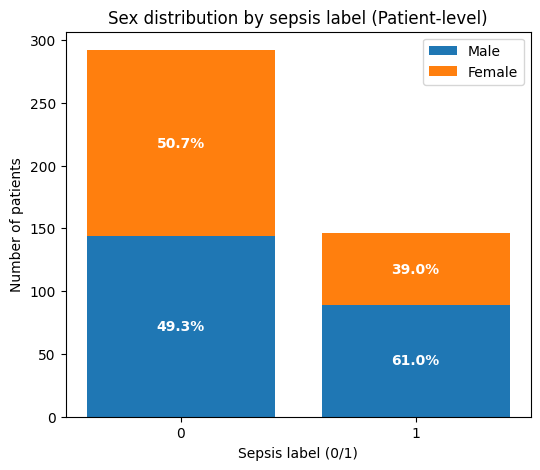
\includegraphics[width=0.9\linewidth]{gender_distribution_patient_level.png}
\caption{Patient-level distribution of biological sex across sepsis and non-sepsis groups.}
\label{fig:gender_distribution}
\end{figure}

\subsubsection{Patient-Aware Splitting}
A patient-aware splitting approach was utilized to avert information leakage between experimental splits. All windows related to a certain patient were exclusively allocated to either the training, validation, or test set. This technique embodies a pragmatic clinical implementation scenario, wherein early warning models are utilized on novel patients instead of subsequent assessments of the same individual \cite{Che2018RNNMissing}.


\subsection{Post-Processing for Practical Early Warning System}

The raw model probabilities were converted into a clinically deployable alerting mechanism using a multi-stage post-processing pipeline. To reduce short-term noise in prediction probabilities, an exponential moving average (EMA) with a smoothing factor of $\alpha \approx 0.20$ was applied. A $k$-of-$n$ detection rule was then used, triggering an alert when $k$ high-probability predictions (e.g., $k=2$) occurred within $n$ consecutive time steps (e.g., $n=3$). Following the initial alert, a refractory period was imposed to suppress subsequent alerts for a fixed duration (e.g., 12 steps).

This design enhances the clinical usability of the proposed early warning system by reducing false positives and alert fatigue.



\subsection{Evaluation Protocol}

The model’s predictions at the patient level will be interpreted in terms of correct and incorrect clinical outcomes. A correct positive (TP) indicates an infant who developed sepsis and for whom the model triggered at least one alert prior to the onset of infection. A false positive (FP) represents an uninfected infant for whom an alert was incorrectly triggered. A true negative (TN) represents an uninfected infant for whom no alert was triggered, while a false negative (FN) indicates an infected infant for whom the model failed to generate any alert before the onset of sepsis.

The model’s performance will be evaluated at both the time window and patient levels, with the primary focus on the patient level (defined as any positive alert per patient) to better reflect real-world clinical benefit.

At the window level, evaluation metrics will include accuracy, precision, recall, F1-score, area under the receiver operating characteristic curve (AU-ROC), and area under the precision–recall curve (AUPRC). Accuracy is defined as
\begin{equation}
\text{Accuracy} = \frac{\text{TP} + \text{TN}}{\text{TP} + \text{TN} + \text{FP} + \text{FN}},
\end{equation}
precision is defined as
\begin{equation}
\text{Precision} = \frac{\text{TP}}{\text{TP} + \text{FP}},
\end{equation}
recall is defined as
\begin{equation}
\text{Recall} = \frac{\text{TP}}{\text{TP} + \text{FN}},
\end{equation}
and the F1-score is defined as
\begin{equation}
\text{F1-score} = 2 \times \frac{\text{Precision} \times \text{Recall}}{\text{Precision} + \text{Recall}}.
\end{equation}

Patient-level evaluation, which represents the primary focus of this study, will comprise sensitivity, specificity, positive predictive value (PPV), negative predictive value (NPV), and lead time. Sensitivity is computed as
\begin{equation}
\text{Sensitivity} = \frac{\text{TP}}{\text{TP} + \text{FN}},
\end{equation}
specificity is defined as as\begin{equation}
\text{Specificity} = \frac{\text{TN}}{\text{TN} + \text{FP}},
\end{equation}
PPV is defined as\begin{equation}
\text{PPV} = \frac{\text{TP}}{\text{TP} + \text{FP}},
\end{equation}
and NPV is defined as\begin{equation}
\text{NPV} = \frac{\text{TN}}{\text{TN} + \text{FN}}.
\end{equation}

Lead time will be calculated as the time difference (in hours) between the first model alert and the true sepsis onset:
\begin{equation}
\text{Lead time} = \frac{t_{\text{event}} - t_{\text{alert}}}{3600}.
\end{equation}

Threshold optimization will be performed on the validation set by prioritizing the F$_2$-score ($\beta = 2$) to emphasize recall over precision, defined as
\begin{equation}
F_\beta = (1 + \beta^2)\frac{\text{Precision} \times \text{Recall}}{\beta^2 \times \text{Precision} + \text{Recall}}.
\end{equation}

Additional evaluation will include probabilistic calibration using the Brier score, defined as
\begin{equation}
\text{Brier score} = \frac{1}{N} \sum_{i=1}^{N} (p_i - o_i)^2,
\end{equation}
where $p_i$ denotes the predicted probability and $o_i \in \{0,1\}$ represents the true outcome.
Reliability diagrams will be used to visualize calibration performance, and optional Platt scaling will be applied using logistic regression on validation probabilities to further improve probability calibration.



\section {EXPECTED RESULTS/OUTPUTS}
The proposed strategy aims to provide an early warning for suspected neonatal sepsis roughly 24 hours prior to commencement, surpassing current models that only identify sepsis within the sepsis window. The model generates a probabilistic forecast for a specified 24-hour period, assigning each data instance a probability that reflects the chance of sepsis onset within the subsequent 24 hours.

“Another expected outcome of using the model will be a clinical and accurate estimation,” as the data provided in the research is segmented in a patient-aware manner (meaning the data here will not be used for training and testing simultaneously); hence, it should produce a reliable and non-exaggerated outcome as opposed to some techniques, which generate data randomly and “proceed to a data leak.” The GRU and LSTM-based models should work well with high sensitivity because, in this research, the aim is to identify as soon as possible while avoiding false alarms to prevent making it impractical and a hindrance to its usability,” as suggested by the researcher.

There is another expected result that includes the production of understandable reports and metrics like the Confusion Matrix, Sensitivity, Specificity, PPV, NPV, alongside the F2 score for supporting early positive detection. There is also the production of a patient-level result where the patient is assessed based on whether they have pressed at least one alert button that more closely relates to what happens in a practical setting compared to the individual window assessments.

Moreover, given the possible lack of proper calibration of the probabilities produced by the model (which might appear overconfident in some instances), the calibration step is anticipated to help in ensuring that the probabilities are more reliable. This will be evident through the Brier score and the reliability graph before and after the calibration step. Lastly, it is anticipated that the post-processing step (which might entail EMA smoothing with k of n as well as the refractory time) will help in lessening the variability of the alarm signal and ensure that the alarm signal does not appear periodically in some instances so that the alarm signal is more logical


\bibliographystyle{ieeetr}
\bibliography{references}
\end{document}
